\documentclass[a4paper]{article}
\usepackage[utf8]{inputenc}
\usepackage{csquotes}
\usepackage[english]{babel}
\usepackage[style = chem-acs]{biblatex}
\addbibresource{citation.bib}
\usepackage{amsmath, mathtools}
\DeclarePairedDelimiter\abs{\lvert}{\rvert}%
\usepackage{dsfont}
\usepackage{graphicx}
\usepackage{float}
\usepackage{subfig}
\usepackage[export]{adjustbox}
%\usepackage[colorinlistoftodos]{todonotes}
\usepackage[margin=1in, left=1.5cm, right=1.5cm, marginparwidth=2.3cm]{geometry}
\usepackage{marginnote}
\usepackage{amssymb}
\usepackage{hyperref}
\usepackage{slashed}
\usepackage{feynmp}
\usepackage{sectsty}
\sectionfont{\sectionrule{3ex}{3pt}{-1ex}{1pt}}
\usepackage{titleps}
\usepackage{fancyhdr}
\usepackage{tcolorbox}
%\tcbset{skin=enhanced}
%\tcbuselibrary{skins}
\usepackage{varwidth}
\usepackage{sidenotes}
%\usepackage{titlesec}
\usepackage{wasysym}
\usepackage{siunitx}
\usepackage{listings}
\usepackage{xcolor}

\definecolor{gray1}{rgb}{0.2,0.2,0.2}
\definecolor{gray2}{rgb}{0.35,0.35,0.35}
\definecolor{gray3}{rgb}{0.5,0.5,0.5}

\lstdefinestyle{mystyle}{   
	commentstyle=\color{gray3},
	keywordstyle=\color{gray2},
	numberstyle=\tiny\color{gray1},
	stringstyle=\color{gray3},
	basicstyle=\ttfamily\footnotesize,
	breakatwhitespace=false,         
	breaklines=true,                 
	captionpos=b,                    
	keepspaces=true,                 
	numbers=left,                    
	numbersep=5pt,                  
	showspaces=false,                
	showstringspaces=false,
	showtabs=false,                  
	tabsize=2
}
\lstset{style=mystyle}

%\renewcommand*{\raggedleftmarginnote}{} % make left margin notes align left
%
\interfootnotelinepenalty=10000
\DeclareGraphicsRule{*}{mps}{*}{}
%\usepackage{feynmf}
\allowdisplaybreaks
% New definition of square root:
% it renames \sqrt as \oldsqrt
\let\oldsqrt\sqrt
% it defines the new \sqrt in terms of the old one
\def\sqrt{\mathpalette\DHLhksqrt}
\def\DHLhksqrt#1#2{%
	\setbox0=\hbox{$#1\oldsqrt{#2\,}$}\dimen0=\ht0
	\advance\dimen0-0.2\ht0
	\setbox2=\hbox{\vrule height\ht0 depth -\dimen0}%
	{\box0\lower0.4pt\box2}}

\pagestyle{fancy}
\fancyhf{}
\fancyhead[R]{page \thepage}
\fancyhead[L]{Experiment 9: Monte Carlo Simulations of Phase Transitions\\ \rightmark}

\numberwithin{equation}{section}

\title{Experiment 9: Monte Carlo Simulations of Phase Transitions}
\author{Chong Tian En}
\date{\today}
\begin{document}
\unitlength = 1mm
\maketitle

\section{Introduction}
\subsection{Ising Phase Transition}
\begin{figure}[H]
	\centering
	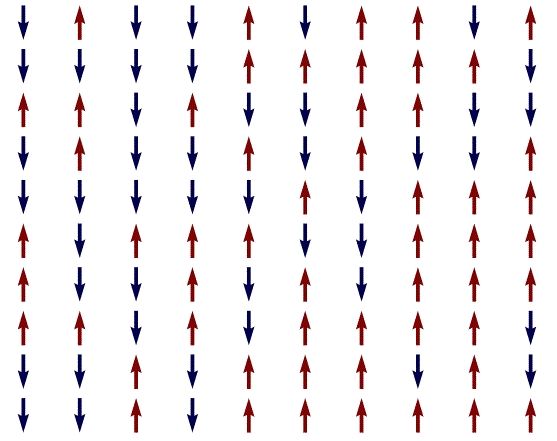
\includegraphics[scale=0.7]{2d_vector.png}
	\caption{Ising 2D $10\times10$}
	\label{fig:ising2d}
\end{figure}
Systems in the universe always tend to lower energy states. If any fluctation can cause them to move towards a lower energy state to achieve stability (i.e. higher probability state), the fluctation can happen very easily. Ising random fluctuation, i.e. spin randomly switching between up and down (see Figure \ref{fig:ising2d} and Figure \ref{fig:illustration} at different temperature $T$), is governed by the probability of flipping spin, which is then governed by its current energy state and its next energy state. When a spin flip can cause its next energy state to be lower than its current one, there is definitely a flipping. For the same temperature $T$, if its next energy state is higher (i.e. lower probability) than its current energy state (i.e. higher probability), it would be harder for spin flip to happen spontaneously, as it requires higher temperature to make up for the drop in probability of the next state. Likewise, if the temperature moves from high $T$ to low $T$, it become less probable for spin flipping, because there is nothing to make up for the difference in probability (see Equation \ref{eq:prob} and the immediate explanation after it). This is where Ising system is trapped in the low energy state as the probabilities to flip diminishes. This low energy, ordered state, where all spins aligned in the same direction is considered as a ferromagnetic phase (Figure \ref{fig:phase}). At high $T$, along the direction $h=0$ where we always have average magnetization $\langle M \rangle=0$, i.e. \# spin up sites = \# spin down sites. The transition between ferromagnetic phase (i.e. ordered phase) to paramagnetic phase (i.e. disordered phase) is 1st order transition due to the discontinuity along $h=0$ (Figure \ref{fig:idealmvst}).
\begin{figure}
	\centering
	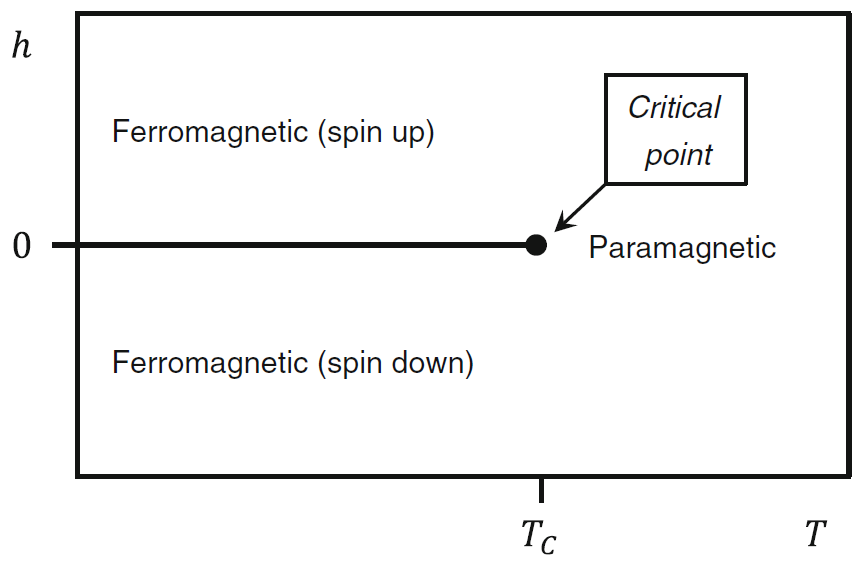
\includegraphics[scale=0.35]{idealphase.png}
	\caption{Ising Phase Diagram as A Function of Field $h$ and Temperature $T$ \cite{softmatter}}
	\label{fig:phase}
\end{figure}
\begin{figure}
	\centering
	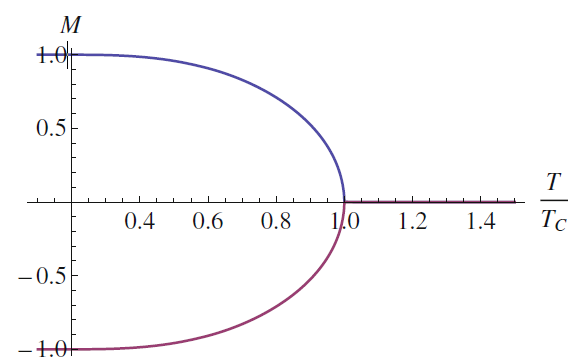
\includegraphics[scale=0.5]{idealmvst.png}
	\caption{Magnetisation per Site $M$ vs Temperature $T$ \cite{softmatter}}
	\label{fig:idealmvst}
\end{figure}
\begin{figure}
	\centering
	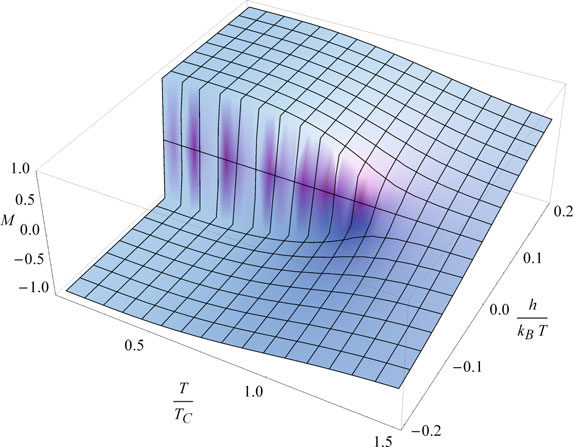
\includegraphics[scale=0.7]{mvsth.png}
	\caption{Magnetisation per Site $M$ vs Temperature $T$ and Field $h$ \cite{softmatter}}
	\label{fig:mvsth}
\end{figure}
If we inspect the 2D surface plot (Figure \ref{fig:mvsth}) of average magnetisation per site $\langle m \rangle$, we can easily identify various discontinuities on the graph, i.e. below $T_c$, we travel across different $h$ along different $T$ (See also Figure \ref{fig:phase}) plus the one we have just mentioned. 1st order phase transition is very obvious, however, 2nd order phase transition is less obvious due to the discontinuity occurring only in its derivatives. i.e. derivatives like heat capacity $C_v$ from average energy $\langle E \rangle$ and susceptibility $\chi_m$ from average magnetisation $\langle M \rangle$. In this experiment, we will inspect both 1st order and 2nd order phase transition of Ising model.

Note that although $\langle m \rangle$ denotes average magnetisation and $\langle M \rangle$ denotes average magnetisation per site (in reference to most textbook), from this point onwards $m$ and $M$ swap their roles, in reference to the lab sheet convention.
\subsection{Monte Carlo Method \cite{lab}}
In this experiment, we create 100 independent simulation runs. For each of these run, we generated $10\times 10$ 2D Ising grid (Figure \ref{fig:ising2d}), and we drop temperature $T$ from 4.0 to 0.1 (Figure \ref{fig:illustration}). So, there are 40 steps for temperature $T$ in total. For each of these step in temperature $T$, we run 1000 Monte Carlo cycles. Each of these cycle constitute 100 $(L^2 = 10\times10)$ moves. Each of these moves will constitute randomly selected site fluctuation (it might flip or it might not), governed by probability mechanism as described below:

\begin{quote}
Let current state of the system be $k$ and the next state be $k'$, and the corresponding probability for the current state and next state would be $P_{k}=\frac{1}{Z}e^{-E_{k}/T}$ and $P_{k'}=\frac{1}{Z}e^{-E_{k'}/T}$ respectively. It also implies we set $k_B=1$. Now, we generate a random ratio $r$ between $[0,1]$ to compare the simulated probability ratio of next potential state to the current state $P_{k'}/P_{k}$. Here, we demand the simulated ratio is to be $> r$ before we do actual spin flipping. Keep in mind that the maximum value for $r$ is 1 but simulated ratio can go over 1. Mathematically, it means:
\begin{align}
\frac{P_{k'}}{P_{k}}&>r\\
\frac{Z^{-1}e^{-E_{k'}/T}}{Z^{-1}e^{-E_{k}/T}}&>r\\
e^{-\frac{\Delta E}{T}}&>r\label{eq:prob}
\end{align}
In our simulation code, we treat $r=1$ separately because the random $r=[0,1]$ generation is actually $r=[0,1)$, i.e. excluding 1. Programmatically and intuitively, it means $r$ is uniform random value between $[0,1]$. If L.H.S. probability ratio $e^{-\frac{\Delta E}{T}}$ is higher, it can cover more range for $r$, i.e. the range $[0,e^{-\frac{\Delta E}{T}}]$, and vice versa. If it is more than 1, it has exceeded $r$'s range, so it met our demand all the time. Since the input parameter for us is temperature $T$, so let's examine $T$:

\begin{quote}
For case $\Delta E$ being positive:

\begin{quote}
	As temperature $T$ gets higher, the probability ratio $e^{-\frac{\Delta E}{T}}$ is getting close to 1 but will not exceed 1. Likewise, if $T$ gets lower, the probability ratio gets lower towards 0.
\end{quote}

For case $\Delta E$ being 0:
\begin{quote}
	It doesn't matter which $T$ (but still undefined at $T=0$, as $0/0$ is undefined), the probability ratio $e^{-\frac{\Delta E}{T}}$ is always 1.
\end{quote}

For case $\Delta E$ being negative:
\begin{quote}
It doesn't matter which $T$, the probability ratio $e^{-\frac{\Delta E}{T}}$ is always $>1$.
\end{quote}

\end{quote}

In the event where our demand is met, we will flip the spin of the site and update the grid. Of course, quantities like energy and magnetisation do change and we need to update accordingly. Although we do update them, we don't collect their data in array until the 100 moves per cycle have been completed, i.e. we only collect at the end of each cycle. With these data, we can proceed to analysis and generate various graphs in this report. Exact program steps are extensively commented in the appendix for understanding.
\end{quote}
\section{Ising Model in Detail}
Each lattice site $s_i$ state is:
$$s_i=+1,-1$$
The hamiltonian (also energy $E$):
$$H=-J\sum_{ij} s_i s_j-h\sum_{i}s_i$$
Here, $J$ is positive. So, when a spin is aligned with its neighbours (i.e. $s_is_j$ being positive), its energy is low and vice versa. Similarly, when a spin is aligned to external field $h$ (i.e. $hs_i$ being positive), its energy is low and vice versa
\subsection{Heat Capacity $C_v$ Derivation}
Heat Capacity $C_v$ is defined as:
$$C_v=\frac{\partial \langle E \rangle}{\partial T}$$
We know:
\begin{equation}\beta = \frac{1}{kT}\label{eq:beta}\end{equation}
Then:
$$-kT^2d\beta=dT$$
Hence with \ref{eq:beta}:
\begin{equation}C_v=-\frac{1}{kT^2}\frac{\partial \langle E \rangle}{\partial \beta}\label{eq:newcv}\end{equation}
The partition function:
$$Z=\sum_{n} e^{-\beta E_n}$$
Partial differentiate with respect to $\beta$:
$$\frac{\partial Z}{\partial B}=\sum_{n} -E_ne^{-\beta E_n}$$
Since $\langle E \rangle$ is defined as:
$$\langle E \rangle=\frac{\sum_{n} E_ne^{-\beta E_n}}{\sum_{n} e^{-\beta E_n}}$$
which means:
$$\langle E \rangle=-\frac{1}{Z}\frac{\partial Z}{\partial B}$$
Similarly, $$\langle E^2 \rangle=\frac{\sum_{n} E_n^2e^{-\beta E_n}}{\sum_{n} e^{-\beta E_n}}=\frac{1}{Z}\frac{\partial^2 Z}{\partial B^2}$$
Then,
\begin{equation}
\langle E^2 \rangle-\langle E \rangle^2=\frac{1}{Z}\frac{\partial^2 Z}{\partial B^2}-\frac{1}{Z^2}\left(\frac{\partial Z}{\partial B}\right)^2=\frac{\partial}{\partial \beta}\left( \frac{1}{Z}\frac{\partial Z}{\partial B}\right)=-\frac{\partial}{\partial \beta}\langle E \rangle\label{eq:evar}
\end{equation}
Finally, with \ref{eq:newcv} and \ref{eq:evar} we have:
$$C_v=\frac{\langle E^2 \rangle-\langle E \rangle^2}{kT^2}$$
\subsection{Susceptibility $\chi_m$ Derivation}
Susceptibility $\chi_m$ is defined as:
\begin{equation}
\chi_m=\frac{\partial \langle M \rangle}{\partial h}\label{eq:sus}
\end{equation}
From hamiltonian, let neighbour interaction $X=\sum_{ij} s_i s_j$ and magnetization $M=\sum_{i} s_i $
Simplified hamiltonian notation:
$$H = -JX-hM$$
Simplified partition function:
$$Z=\sum e^{-\beta (-JX-hM)}=\sum e^{\beta(JX+hM)}$$
Partial differentiate with respect to $h$:
$$\frac{\partial Z}{\partial h}=\beta\sum Me^{\beta(JX+hM)}$$
Partial differentiate again with respect to $h$:
$$\frac{\partial ^2 Z}{\partial h^2}=\beta^2\sum M^2e^{\beta(JX+hM)}$$
Similarly, average magnetization $\langle M \rangle$:
$$\langle M \rangle=\frac{\sum Me^{\beta(JX+hM)}}{\sum e^{\beta(JX+hM)}}=\frac{1}{\beta Z}\frac{\partial Z}{\partial h}$$
And average magnetization squared $\langle M^2 \rangle$:
$$\langle M^2 \rangle=\frac{\sum M^2e^{\beta(JX+hM)}}{\sum e^{\beta(JX+hM)}}=\frac{1}{\beta^2 Z}\frac{\partial^2 Z}{\partial h^2}$$
Then,
$$\langle M^2 \rangle-\langle M \rangle^2=\frac{1}{\beta^2 Z}\frac{\partial^2 Z}{\partial h^2}-\left(\frac{1}{\beta Z}\frac{\partial Z}{\partial h} \right)^2=\frac{\partial}{\partial h}\left(\frac{1}{\beta^2 Z}\frac{\partial Z}{\partial h}\right)=\frac{1}{\beta}\frac{\partial \langle M \rangle}{\partial h}$$
Together with \ref{eq:sus} and \ref{eq:beta} we have:
$$\chi_m=\frac{\langle M^2 \rangle-\langle M \rangle^2}{kT}$$
Since we only concern about intensive quantity average magnetization per site $m=M/N$, finally we have:
$$\chi_m=\frac{\langle m^2 \rangle-\langle m \rangle^2}{kT}$$
\section{Results}
\subsection{Question 1}
\begin{figure}[H]
	\centering
	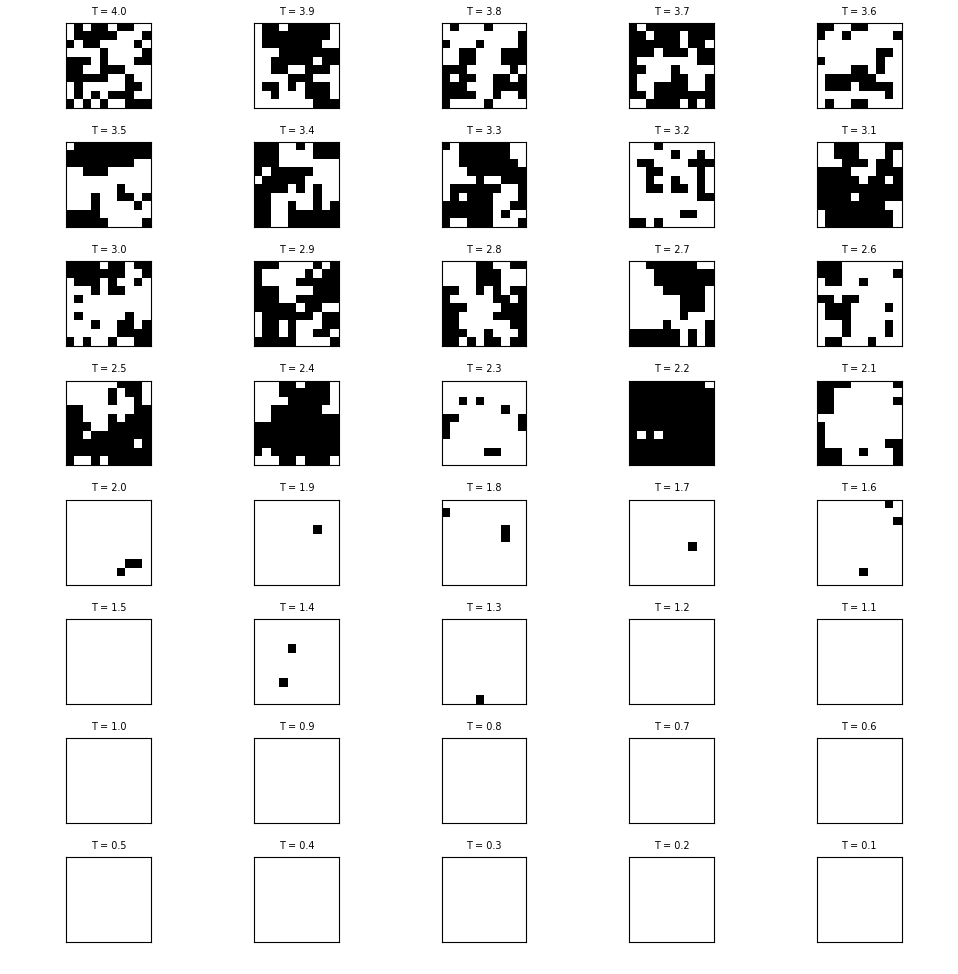
\includegraphics[scale=0.7]{illustration.png}
	\caption{Illustration of the System at Selected Temperatures (white for site with spin up "$+1$", black for site with spin down "$-1$")}
	\label{fig:illustration}
\end{figure}
\subsection{Question 2}
\begin{figure}[H]
	\centering
	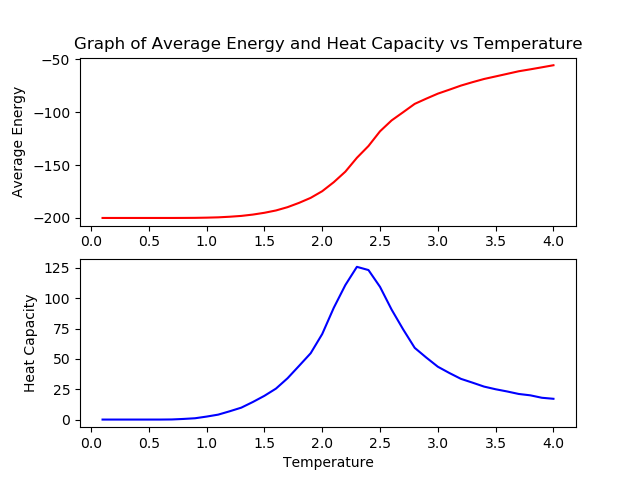
\includegraphics[scale=0.7]{ecvvst.png}
	\caption{Average Energy $\langle E \rangle$ and the Specific Heat $C_v$ as A Function of the Temperature $T$}
	\label{fig:ecvvst}
\end{figure}
\subsection{Question 3}
\begin{figure}[H]
	\centering
	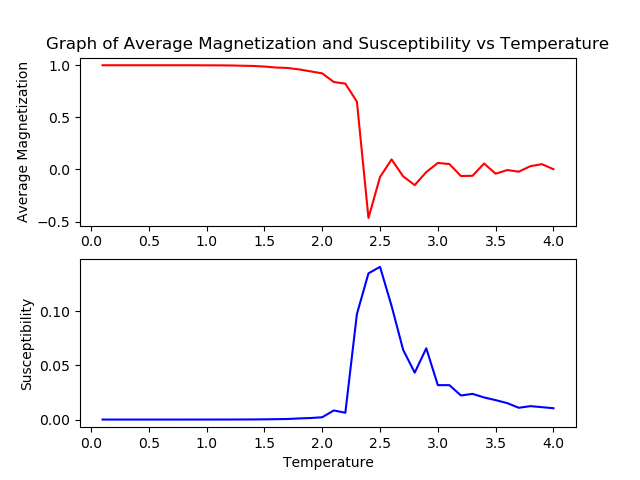
\includegraphics[scale=0.7]{mxvst.png}
	\caption{Average Magnetization $\langle m \rangle$ and the Susceptibility $\chi_m$ as A Function of the Temperature $T$}
	\label{fig:mxvst}
\end{figure}
\subsection{Question 4}
\begin{figure}[H]
	\centering
	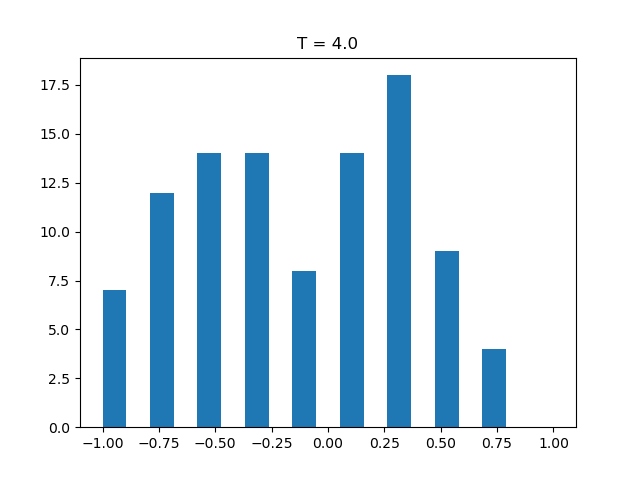
\includegraphics[scale=0.7]{probdist1.png}
	\caption{Probability Distribution of Average Magnetisation Per Spin $m_k(T)$ at $100^{th}$ Simulation at Temperature $T=4.0$}
	\label{fig:probdist1}
\end{figure}
\begin{figure}[H]
	\centering
	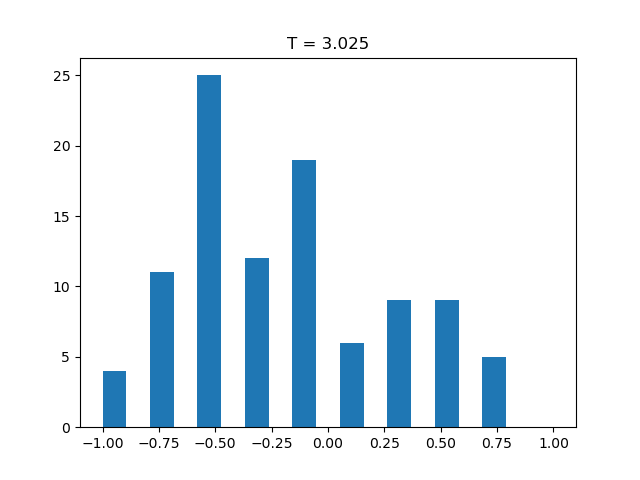
\includegraphics[scale=0.7]{probdist2.png}
	\caption{Probability Distribution of Average Magnetisation Per Spin $m_k(T)$ at $100^{th}$ Simulation at Temperature $T=3.025$}
	\label{fig:probdist2}
\end{figure}
\begin{figure}[H]
	\centering
	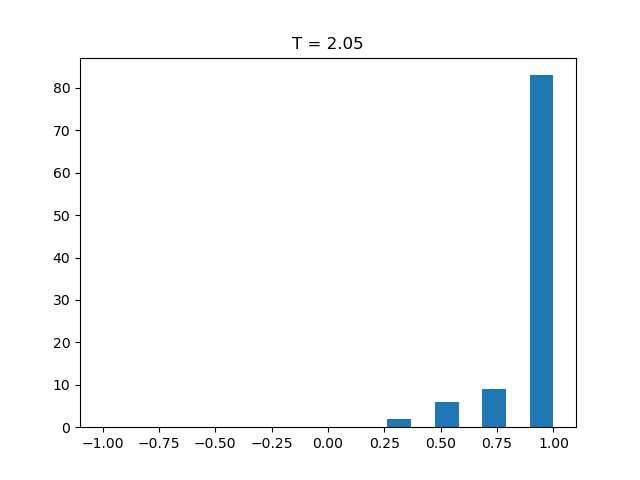
\includegraphics[scale=0.7]{probdist3.png}
	\caption{Probability Distribution of Average Magnetisation Per Spin $m_k(T)$ at $100^{th}$ Simulation at Temperature $T=2.05$}
	\label{fig:probdist3}
\end{figure}
\begin{figure}[H]
	\centering
	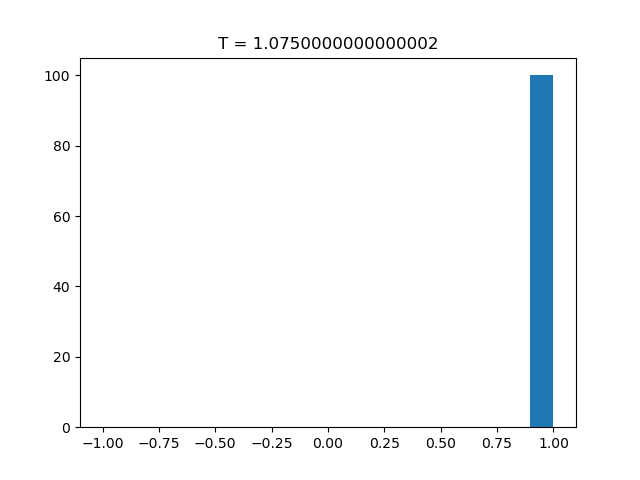
\includegraphics[scale=0.7]{probdist4.png}
	\caption{Probability Distribution of Average Magnetisation Per Spin $m_k(T)$ at $100^{th}$ Simulation at Temperature $T=1.075$}
	\label{fig:probdist4}
\end{figure}
\begin{figure}[H]
	\centering
	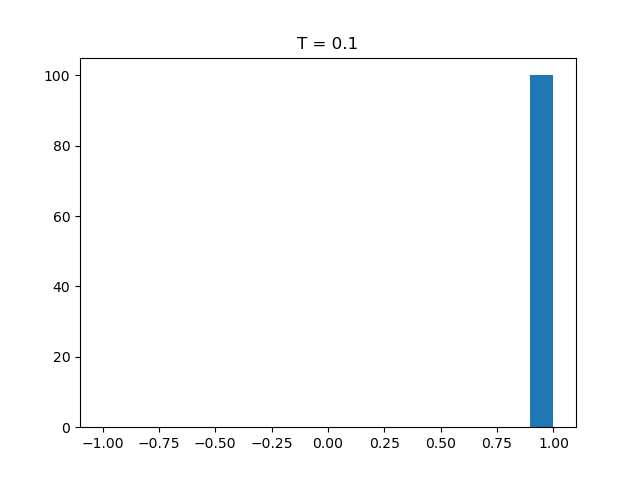
\includegraphics[scale=0.7]{probdist5.png}
	\caption{Probability Distribution of Average Magnetisation Per Spin $m_k(T)$ at $100^{th}$ Simulation at Temperature $T=0.1$}
	\label{fig:probdist5}
\end{figure}
\section{Discussion}
\subsection{Question 1}
From Figure \ref*{fig:illustration}, at high $T$ the spins are highly randomized and almost equal in number in up and down. Heavy fluctuation occurs around $T=T_c\approx2.3$ where mostly down at $T=2.4$ suddenly flipped to mostly up at $T=2.3$ then back to mostly down at $T=2.2$ before finally settling on mostly up at $T=2.1$. Once it passed $T_c$, it progressively gets stuck at all spin up as it tends towards $T=0.1$.
\subsection{Question 2}
We expect average energy $\langle E \rangle$ to increase as temperature $T$ increases and the 2nd order phase transition happen where the gradient become discontinous, even when the original curve is continous. We do observe  that $\langle E \rangle$ increases the most at $T_c$. Its increase will be more dramatic with even larger simulation matrix (i.e. $\gg 10\times10$). Since heat capacity $C_v$ is just $\frac{d\langle E \rangle}{dT}$, we have the gradient of the first graph. At $T=T_c\approx2.3$, heat capacity $C_v$ diverges, this translate to 2nd order phase transition. In the result, we observe $C_v$ sort of diverges at $T_c$ as the gradient at the peak is not exactly sharp. Even larger simulation matrix can result in a more obvious narrow spike.
\subsection{Question 3}
First order phase transition not obvious in the simulation due to just 1 simulation. However, average magnetization per site $\langle m \rangle$, closely resembles the ideal case in our introduction. Susceptibility is less obvious not just due to 1 simulation, but also that it is not differentiated with respect to $T$ but with respect to $h$, where $h=0$ in our case. 
\subsection{Question 4}
We expect probability distribution to be fairly uniform at high $T$, but at around $T_c$, it should be tending towards oneside (left or right) and stays there till lowest $T$. This is because there is spontaneous symmetry breaking in low temperature, as the average magnetisation per site $\langle m \rangle$ tending towards lowest temperature is either $+1$ or $-1$ once the system crosses $T_c$ along $h=0$. When the symmetry is not broken, the system only has one symmetrical lowest point and does not have  2 opposite lowest points, which system can fall onto either one and trap there. Indeed, we observed that there are lots of fluctuation around $T_c$ before our system pick $\langle m \rangle=+1$ to settle on Figure \ref{fig:mxvst}, where average magnetisation per spin $\langle m \rangle$ stuck at +1. On a separate simulation, it does pick $\langle m \rangle=-1$ too.
\section{Conclusion}
Monte Carlo method is very useful in simulating Ising model. In real world, Monte Carlo method can simulate systems with random fluctuation, but still obey probabilities that are subjected to certain rules. The real world application includes but not limited to mathematics, science, engineering, business, finance, law, and search and rescue \cite{wiki}.
\printbibliography
\section{Appendix}
\lstinputlisting[language=Python, caption=Monte Carlo Python Simulation File]{Code2.py}
\begin{table}[ht]
	\centering
	\subfloat[Temperature $T$ and Average Energy $\langle E \rangle$][Temperature $T$ and Average Energy $\langle E \rangle$]{
		\begin{tabular}[t]{cc}
			\hline
			Temperature $T$ & Average Energy $\langle E \rangle$\\
			\hline
			\hline
			0.1 & -200.000000 \\
			0.2 & -200.000000 \\
			0.3 & -200.000000 \\
			0.4 & -200.000000 \\
			0.5 & -200.000000 \\
			0.6 & -199.999840 \\
			0.7 & -199.994640 \\
			0.8 & -199.959360 \\
			0.9 & -199.893520 \\
			1.0 & -199.704240 \\
			1.1 & -199.412080 \\
			1.2 & -198.836560 \\
			1.3 & -198.059360 \\
			1.4 & -196.803520 \\
			1.5 & -195.107840 \\
			1.6 & -192.911920 \\
			1.7 & -189.789280 \\
			1.8 & -185.712000 \\
			1.9 & -181.001280 \\
			2.0 & -174.703200 \\
			2.1 & -166.183200 \\
			2.2 & -156.250480 \\
			2.3 & -143.124320 \\
			2.4 & -131.995200 \\
			2.5 & -118.074880 \\
			2.6 & -107.815280 \\
			2.7 & -100.040400 \\
			2.8 & -92.166720 \\
			2.9 & -87.222960 \\
			3.0 & -82.502160 \\
			3.1 & -78.741600 \\
			3.2 & -74.871920 \\
			3.3 & -71.648160 \\
			3.4 & -68.634480 \\
			3.5 & -66.222640 \\
			3.6 & -63.780000 \\
			3.7 & -61.335120 \\
			3.8 & -59.519280 \\
			3.9 & -57.600480 \\
			4.0 & -55.648160 \\
			\hline
	\end{tabular}}
	\qquad
	\subfloat[Temperature $T$ and Heat Capacity $C_v$][Temperature $T$ and Heat Capacity $C_v$]{
		\begin{tabular}[t]{cc}
			\hline
			Temperature $T$ & Heat Capacity $C_v$\\
			\hline
			\hline
			0.1 & 0.000000 \\
			0.2 & 0.000000 \\
			0.3 & 0.000000 \\
			0.4 & 0.000000 \\
			0.5 & 0.000000 \\
			0.6 & 0.003548 \\
			0.7 & 0.089029 \\
			0.8 & 0.515550 \\
			0.9 & 1.076819 \\
			1.0 & 2.455944 \\
			1.1 & 4.059295 \\
			1.2 & 6.840299 \\
			1.3 & 9.823511 \\
			1.4 & 14.490010 \\
			1.5 & 19.583755 \\
			1.6 & 25.538257 \\
			1.7 & 34.054436 \\
			1.8 & 44.307861 \\
			1.9 & 54.682800 \\
			2.0 & 70.551703 \\
			2.1 & 92.192352 \\
			2.2 & 110.924838 \\
			2.3 & 125.958214 \\
			2.4 & 123.304323 \\
			2.5 & 109.434761 \\
			2.6 & 90.715857 \\
			2.7 & 74.367163 \\
			2.8 & 59.134921 \\
			2.9 & 51.137181 \\
			3.0 & 43.585194 \\
			3.1 & 38.384421 \\
			3.2 & 33.567535 \\
			3.3 & 30.439533 \\
			3.4 & 27.182868 \\
			3.5 & 24.992956 \\
			3.6 & 23.161960 \\
			3.7 & 21.109158 \\
			3.8 & 19.985494 \\
			3.9 & 17.973747 \\
			4.0 & 17.128732 \\
			\hline
	\end{tabular}}
	\caption{Table of Simulation Data}
\end{table}
\begin{table}[ht]
	\ContinuedFloat
	\centering
	\subfloat[Temperature $T$ and Average Magnetization $\langle m \rangle$][Temperature $T$ and Average Magnetization $\langle m \rangle$]{
		\begin{tabular}[t]{cc}
			\hline
			Temperature $T$ & Average Magnetization $\langle m \rangle$\\
			\hline
			\hline
			0.1 & 1.000000 \\
			0.2 & 1.000000 \\
			0.3 & 1.000000 \\
			0.4 & 1.000000 \\
			0.5 & 1.000000 \\
			0.6 & 1.000000 \\
			0.7 & 1.000000 \\
			0.8 & 0.999920 \\
			0.9 & 0.999680 \\
			1.0 & 0.999080 \\
			1.1 & 0.998720 \\
			1.2 & 0.997920 \\
			1.3 & 0.995440 \\
			1.4 & 0.993160 \\
			1.5 & 0.987520 \\
			1.6 & 0.977920 \\
			1.7 & 0.973840 \\
			1.8 & 0.960000 \\
			1.9 & 0.940880 \\
			2.0 & 0.922120 \\
			2.1 & 0.839200 \\
			2.2 & 0.823360 \\
			2.3 & 0.650480 \\
			2.4 & -0.465480 \\
			2.5 & -0.072840 \\
			2.6 & 0.096400 \\
			2.7 & -0.066240 \\
			2.8 & -0.150000 \\
			2.9 & -0.025080 \\
			3.0 & 0.062600 \\
			3.1 & 0.051520 \\
			3.2 & -0.063000 \\
			3.3 & -0.060880 \\
			3.4 & 0.057240 \\
			3.5 & -0.040960 \\
			3.6 & -0.005800 \\
			3.7 & -0.021240 \\
			3.8 & 0.031200 \\
			3.9 & 0.050920 \\
			4.0 & 0.002280 \\
			\hline
	\end{tabular}}
	\qquad
	\subfloat[Temperature $T$ and Susceptibility $\chi_m$ $C_v$][Temperature $T$ and Susceptibility $\chi_m$]{
		\begin{tabular}[t]{cc}
			\hline
			Temperature $T$ & Susceptibility $\chi_m$\\
			\hline
			\hline
			0.1 & -0.000000 \\
			0.2 & -0.000000 \\
			0.3 & -0.000000 \\
			0.4 & -0.000000 \\
			0.5 & -0.000000 \\
			0.6 & -0.000000 \\
			0.7 & -0.000000 \\
			0.8 & 0.000002 \\
			0.9 & 0.000007 \\
			1.0 & 0.000021 \\
			1.1 & 0.000025 \\
			1.2 & 0.000042 \\
			1.3 & 0.000079 \\
			1.4 & 0.000107 \\
			1.5 & 0.000205 \\
			1.6 & 0.000360 \\
			1.7 & 0.000530 \\
			1.8 & 0.001039 \\
			1.9 & 0.001440 \\
			2.0 & 0.002144 \\
			2.1 & 0.008408 \\
			2.2 & 0.006305 \\
			2.3 & 0.097568 \\
			2.4 & 0.135162 \\
			2.5 & 0.141207 \\
			2.6 & 0.105009 \\
			2.7 & 0.064454 \\
			2.8 & 0.043372 \\
			2.9 & 0.065895 \\
			3.0 & 0.031828 \\
			3.1 & 0.031805 \\
			3.2 & 0.022253 \\
			3.3 & 0.023757 \\
			3.4 & 0.020440 \\
			3.5 & 0.017962 \\
			3.6 & 0.015230 \\
			3.7 & 0.010896 \\
			3.8 & 0.012405 \\
			3.9 & 0.011465 \\
			4.0 & 0.010475 \\
			\hline
	\end{tabular}}
	\caption{Table of Simulation Data (Continued)}
\end{table}
\end{document}